\documentclass[a4paper]{article}
\usepackage{interspeech2013,amssymb,amsmath,epsfig}
\setcounter{page}{1}
\sloppy		% better line breaks
\ninept
%SM below a registered trademark definition
\def\reg{{\rm\ooalign{\hfil
     \raise.07ex\hbox{\scriptsize R}\hfil\crcr\mathhexbox20D}}}

%% \newcommand{\reg}{\textsuperscript{\textcircled{\textsc r}}}
\title{Relationships Between Prosodic-Linguistic Features and High-Level Descriptors of Speed Dates}

%%%%%%%%%%%%%%%%%%%%%%%%%%%%%%%%%%%%%%%%%%%%%%%%%%%%%%%%%%%%%%%%%%%%%%%%%%
%% If multiple authors, uncomment and edit the lines shown below.       %%
%% Note that each line must be emphasized {\em } by itself.             %%
%% (by Stephen Martucci, author of spconf.sty).                         %%
%%%%%%%%%%%%%%%%%%%%%%%%%%%%%%%%%%%%%%%%%%%%%%%%%%%%%%%%%%%%%%%%%%%%%%%%%%
%\makeatletter
%\def\name#1{\gdef\@name{#1\\}}
%\makeatother
%\name{{\em Firstname1 Lastname1, Firstname2 Lastname2, Firstname3 Lastname3,}\\
%      {\em Firstname4 Lastname4, Firstname5 Lastname5, Firstname6 Lastname6,
%      Firstname7 Lastname7}}
%%%%%%%%%%%%%%% End of required multiple authors changes %%%%%%%%%%%%%%%%%

\makeatletter
\def\name#1{\gdef\@name{#1\\}}
\makeatother
\name{{\em Sidd Jagadish$^\ast$, Ranjay Krishna$^\ddagger$, Gabriele Carotti-Sha$^\mp$}}
\address{{\small \tt siddj@stanford.edu, rak248@stanford.edu, gcarotti@stanford.edu}\\
$\ast$Department of Statistics, Stanford University \\
  $^\ddagger$Department of Computer Science, Stanford University\\
  $^\mp$ Symbolic Systems, Stanford University\\
}

%
\begin{document}
\maketitle
%

\begin{abstract}
We extract lexical and prosodic features of speech from 1493 speed dates at Stanford University.  Each speed date is accompanied by information about what each participant thought of the other, including 1-10 assessments of courteousness and funniness.  Here, we investigate prediction of these assessments from lexical and prosodic features.  We find that for many labels, lexical and prosodic features can powerfully predict our high-level descriptors.
\end{abstract}

\noindent{\bf Index Terms}: Prosody, Speed Date, AdaBoost, Gender differences in prosody, factor analysis, courteous, funny

%

\section{Introduction}

\section{Related Works}


\section{Data}
We were given, courtesy of Jurafsky (2013), a dataset consisting of 1980 (CHECK THIS VALUE) heterosexual speed dates. For each date, we have two .wav files corresponding to the microphones attached to each participant.  We also have high-level descriptors of each participant, including their height, weight, and ethnicity.  In addition to this, for each participant, we have 1-10 assessments of various qualities of both themselves and each other person they went on a speeddate with, including funniness and courteousness.

\subsection{Feature Extraction}

\subsubsection{Prosodic Feature}
Prosodic features were extracted using openSMILE.  Lexical features were extracted in Python, with the help of the LIWC dictionary.  

\subsubsection{Lexical Feature}

\subsubsection{LIWC Feature}

\subsubsection{Accomodation Feature}
Accommodation features include rate of 

\section{Exploratory Analysis}
Before attempting to classify speakers as funny or not, we examine the underlying dimensions along which the data varies.  To do, so we use exploratory factor analysis. To determine the number of factors, we use a scree test and various non-graphical measures, including parallel analysis and an optimal coordinates test, as described in (CITE).  We find an optimal number of factors $k = 5$ for both males and females, conducted separately.  Figure 1 shows the two scree plots.

\begin{figure}[t]
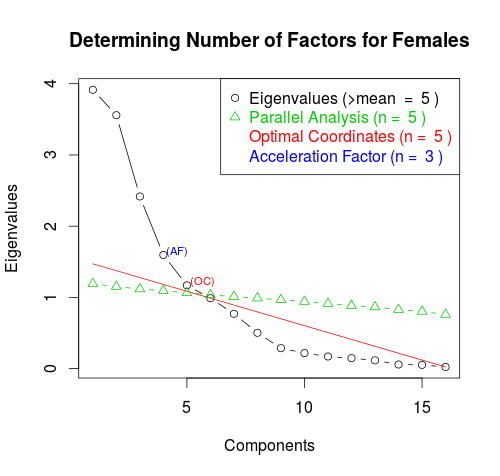
\includegraphics[width = 3.5cm]{graphics/ScreeFem.png}
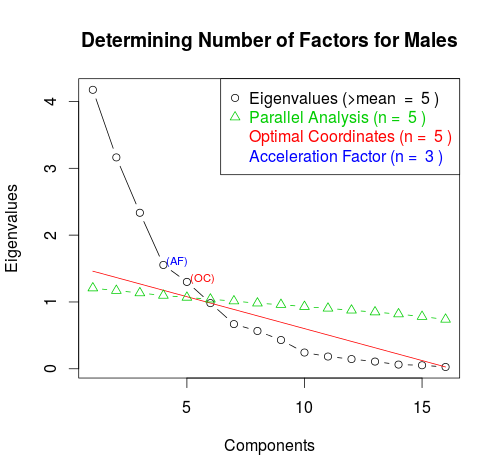
\includegraphics[width = 3.5cm]{graphics/ScreeMale.png}
\caption{{\it Determining Number of Factors}}  
\end{figure}

Interestingly, although we find that the various factors for male and female speech are similar, they explain different amounts of variation in the data.  For males, the first factor reflects high intensity values and low intensity variation, explaining   

\section{Methodology}

\section{Classification Results}

\section{Analysis}

\section{Page layout and style}

\subsection{Figures}

All figures must be centered on the column (or page, if the figure spans 
both columns).
Figure captions should follow each figure and have the format given in 
Figure~\ref{spprod}.

Figures should preferably be line drawings. If they contain gray 
levels or colors, they should be checked to print well on a 
high-quality non-color laser printer.

Graphics (i.e. illustrations, figures) must not use stipple fill
patterns because they will not reproduce properly in Acrobat PDF.
Please use only SOLID FILL COLORS.

Figures which span 2 columns (i.e. occupy full page width) should be
placed at the top or bottom of the page.



\subsection{Tables}

An example of a table is shown as Table \ref{table1}. Somewhat 
different styles are allowed according to the type and purpose of the 
table. The caption text may be above or below the table.

\begin{table} [t,h]
\caption{\label{table1} {\it This is an example of a table.}}
\vspace{2mm}
\centerline{
\begin{tabular}{|c|c|}
\hline
ratio & decibels \\
\hline  \hline
1/1 & 0 \\
2/1 & $\approx 6$ \\
3.16 & 10 \\
10/1 & 20 \\ 
1/10 & -20 \\
100/1 & 40 \\
1000/1 & 60 \\
\hline
\end{tabular}}
\end{table}

\subsection{Equations}

Equations should be placed on separate lines and numbered. Examples 
of equations are given below.
Particularly,
%
%\vspace{-3mm}
\begin{equation}
x(t) = s(f_\omega(t))
\label{eq1}
\end{equation}
where \(f_\omega(t)\) is a special warping function
\begin{equation}
f_\omega(t)=\frac{1}{2\pi j}\oint_C \frac{\nu^{-1k}d\nu}
{(1-\beta\nu^{-1})(\nu^{-1}-\beta)}
\label{eq2}
\end{equation}
A residue theorem states that
\begin{equation}
\oint_C F(z)dz=2 \pi j \sum_k Res[F(z),p_k]
\label{eq3}
\end{equation}
Applying (\ref{eq3}) to (\ref{eq1}), 
it is straightforward to see that
\begin{equation}
1 + 1 = \pi
\label{eq4}
\end{equation}

Finally we have proven the secret theorem of all speech sciences. 
No more math is needed to show how useful the result is! 

\begin{figure}[t]
\centerline{\epsfig{figure=figure,width=80mm}}
\caption{{\it Schematic diagram of speech production.}}  
\label{spprod}
\end{figure}

\subsection{References}

The reference format is the standard IEEE one.
References should be numbered in order of appearance, 
for example \cite{ES1}, \cite{ES2}, and \cite{ES3}. 

\section{Future Work}


\section{Conclusions}


\section{Acknowledgements}
We thank Dan Jurafsky for giving us access to the Speed Dating Dataset and for his continued guidance during this project.

\newpage
%
\eightpt
\bibliographystyle{IEEEtran}
\begin{thebibliography}{10}
\bibitem[1]{ES1} Smith, J. O. and Abel, J. S., 
``Bark and {ERB} Bilinear Transforms'', 
IEEE Trans. Speech and Audio Proc., 7(6):697--708, 1999.  
\bibitem[2]{ES2} Soquet, A., Saerens, M. and Jospa, P.,``Acoustic-articulatory
inversion'', in T. Kohonen [Ed], Artificial Neural Networks, 371-376,
Elsevier, 1991.
\bibitem[3]{ES3} Stone, H.S., ``On the uniqueness of the convolution theorem
for the Fourier transform'', NEC Labs. Amer. Princeton, NJ. 
Online: http://citeseer.ist.psu.edu/176038.html, accessed on 19 Mar 2008.
\end{thebibliography}
\end{document}
